% Estmal alles in einem .tex file, evtl später in mehr aufspalten ...

\section{Introduction}
Presslufthammer is an attempt at developing a prototype of the Dremel Query
System \cite{melnik2010dremel} developed by Google. Dremel is purportedly the
technology that powers the Google BigQuery \cite{bigquery} system. We will
therefore mention it in this report and also reference the BigQuery online
documentation, when talking about features of the Presslufthammer system
and comparing the functionality.

Dremel is a system that allows relational queries\footnote{BigQuery
(and Dremel) use a query language that is very similar to SQL: 
\url{https://developers.google.com/bigquery/docs/query-reference}.} to be
performed on a cluster of machines on very large datasets. The focus here
is on aggregation queries that have very small result sets compared to the
processed amounts of data and that are ``interactive'', meaning that the
results are available quick enough to work with the system interactively.

For more in-depth background information about Dremel and BigQuery you should
consult the paper or the documentation respectively. We will only highlight
the key components and difficulties in the following sections.

\subsection{Division of Work}

The Dremel systems has a very modular architecture, making it easy to share the
work. We identified to following key components (The person working on that
particular component is mentioned in parentheses):

\begin{itemize}
  \item Network architecture (Fabian)
  \item Columnar data representation (Aljoscha)
  \item Parsing, analysis, transformation and execution of Queries (Aljoscha)
  \item Utilities and stuff (Aljoscha, Fabian)
\end{itemize}

Each of these described in their own section respectively.

\subsection{Some Notes}
The Presslufthammer system is implemented in Java and makes use of several tools
and libraries to realise different features:

\begin{itemize}
  \item Maven \cite{maven} for the build system
  \item ANTLR \cite{antlr} for implementing the query parser
  \item Netty \cite{netty} for the network layer
  \item slf4j \cite{slf4j} for logging
  \item Jetty \cite{jetty} as web server for a front end and
  \item Google guava libraries \cite{guava} because they are just plain helpful
\end{itemize}

All package names of Presslufthammer are of the form\\
\texttt{de.tuberlin.dima.presslufthammer.*},\\
but we omit the first part in the following sections for the sake of simplicity,
i.e. package \texttt{data} instead of package
\texttt{de.tuberlin.dima.presslufthammer.data}.

\section{Network Architecture}
  This section presents the components that comprise the network architecture
  we implemented to create the Presslufthammer system.
  All classes of the network architecture are located in the \texttt{transport}
  package and it's child packages \texttt{messages} and \texttt{util}.
  
  
  \subsection{Looking at Dremel}
    First take a look at the way the Dremel \cite{melnik2010dremel} system is
    organised.
    It consists of a multi-layered architecture including:
    \begin{itemize}
      \item A client to provide the user interface
      \item A root server to communicate with the client as well as to dispatch
        queries
      \item Multiple intermediate servers
      \item Multiple leaf servers to access the data and execute queries on it
      \item And finally a seperate storage layer holding the data
    \end{itemize}
    This is illustrated in \figref{netarch}.
    \begin{figure}[ht]
      \centering
      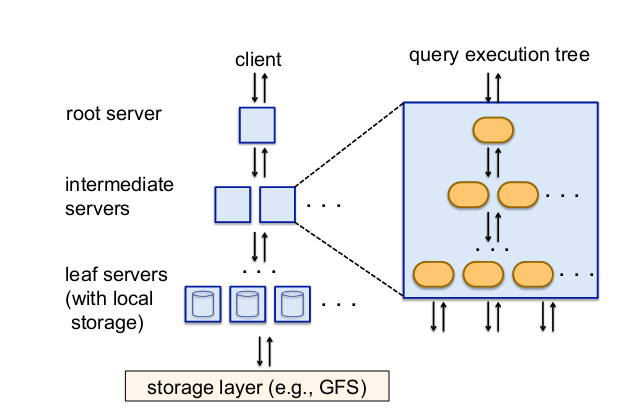
\includegraphics[width=.7\textwidth]{images/net-arch}
      \caption{The overall architecture of Dremel\cite{melnik2010dremel}}
      \label{fig:netarch}
    \end{figure}


  \subsection{Coordinator Leaf Architecture}
    For the first milestone, we implemented only a root server
    (\texttt{Coordinator}) and the leaf servers (\texttt{Leafs}),
    omitting the intermediate layer.
    This allowed us to concentrate on more basic communication features,
    such as the passing of queries and resulting data.
    \subsubsection{The Coordinator Role}
      The \texttt{Coordinator} node provides an entry point for all other nodes
      in the system.
      It is the central object used to organise the network nodes.
      Without an intermediate layer, the \texttt{Coordinator} manages all
      \texttt{Leafs} itself. It splits the queries based on available tablet
      information and distributes the parts of a query among the \texttt{Leafs}.
    
    
  \subsection{Slave Architecture}
    We then went on to implement an additional set of nodes, based on the
    idea of multi purpose nodes that can take both the role of a leaf
    and an intermediate server depending on the situation.
    These nodes are called \texttt{Slaves} and work in conjunction with the
    \texttt{SlaveCoordinator}, that replaces the aforementioned 
    \texttt{Coordinator} as root server.
    \texttt{Slaves} arrange themselves in a n-ary tree.
    The degree of the tree is configurable at instantiation
    and can differ between instances.
    This way, it is possible to create subtrees of higher or lower degree
    than the rest of the tree.


  \subsection{Client Nodes}
    The Presslufthammer system allows for multiple Client nodes to connect.
    For testing and presentation of our prototype we implemented two such
    clients.
    \begin{itemize}
      \item The first is a basic client that we use to provide command
            line access to the querying system.
            It's main purpose is the facilitating of tests.
      \item The second provides the same functionality as the first,
            but uses Jetty \cite{jetty} to provide a html based web
            interface.
            It can provide remote access to users, without the need
            to execute any client-side Java code.
    \end{itemize}
    These clients use the QueryParser to parse entered queries and obtain
    an internal representation of these.


  \subsection{Further Details}
    The network communication was realised using the Netty framework.
    All implemented nodes use the \texttt{GenericHandler} and
    \texttt{GenericPipelineFactory} classes, based on standard Netty classes,
    to send and receive messages.
    The system knows three types of network messages.
    \begin{itemize}
      \item \texttt{SimpleMessages} provide the means to transmit meta data
      \item \texttt{QueryMessages} contain the query objects used by
        Presslufthammer and
      \item \texttt{TabletMessages} encapsulate the result data of a query.
    \end{itemize}


\section{Columnar Data Representation}
The novel aspect of the Dremel system is that it stores hierarchical nested
records in a columnar format and therefore makes queries that only
access some of the fields of a record very efficient because only a small
part of the data has to be read.

We will not explain the special columnar data format here but only give
some details of how things are implemented in the Presslufthammer
system. A complete elaboration would be outside the scope if this
rather short report and the Dremel paper \cite{melnik2010dremel}
explains the format and the necessary algorithms very nicely.

There are three parts that deal with data and we will elaborate each in
turn in the following:

\begin{description}
  \item[Hierarchical Data] This part deals with hierarchical nested records, this
    is the format in which data is imported into the system and also in which
    the user is probably expecting the query results to be.
  \item[Columnar Data] This part is concerned with the efficient format that is
    used internally to facilitate queries at interactive speeds.
  \item[Transformation] The data obviously needs to be transformed between the two
    representations, this is what the transformation part is about.
\end{description}

All code that works with data is located in the \texttt{data} package,
some common classes and the transformation code is directly in \texttt{data},
the code that deals with the columnar format is in \texttt{data.columnar},
and the code for hierarchical data is in \texttt{data.hierarchical}.

\subsection{Auxiliary Code}
For Presslufthammer to be able to work with data a schema description is
necessary. We use the format used by Google Protobuffers, just as
the Dremel system does, for the schema description.\footnote{Google BigQuery
\cite{bigquery} does not use Protobuffer schema descriptions but instead uses
JSON to describe the schema.}\footnote{Internally neither code nor concepts
of Presslufthammer have anything in common with Google Protobuffers.}
An example schema description (taken from the Dremel paper \cite{melnik2010dremel}
is given in \lstref{document-schema}.

\begin{lstlisting}[float=htpb,label={lst:document-schema},caption={Protobuf-like schema definition for the documents data-set.}]
package Document;
message Document {
      required int64 DocId = 1;
      message Links {
            repeated int64 Backward = 1;
            repeated int64 Forward = 2; }
      optional Links Links = 2;
      message Name {
            message Language {
                  required string Code = 1;
                  optional string Country = 2; }
            repeated Language Language = 1;
            optional string Url = 2; }
      repeated Name Name = 3; }
\end{lstlisting}

For working with schema descriptions we have \texttt{SchemaNode} for
representing a schema as a tree data-structure, the enum \texttt{PrimitiveType}
for representing the primitive types in a schema and \texttt{ProtobufSchemaHelper}
for loading/parsing a schema description in the Protobuf format to a
tree of \texttt{SchemaNodes} and also for the reverse process.

\subsection{Hierarchical Data}
Most of the code that deals with hierarchical data is concerned with
delivering the information that is required by the column striping and record
assembly algorithms described in the appendix of the Dremel paper \cite{melnik2010dremel}.
All mentioned classes except \texttt{Field} are actually interfaces and the
implementation for hierarchical data in JSON format is in the package
\texttt{data.hierarchical.json}. We do not mention the JSON classes here
because they are just straightforward implementations of the described
functionality.

We have class \texttt{Field} that represents one field in the hierarchical
record. It provides methods to retrieve the \texttt{SchemaNode} of that
particular field and to write the contained value to a column in
the columnar data representation.\footnote{It writes the value to a
\texttt{ColumnWriter}, see \secref{columnar} for details on that.} \texttt{Field}
is actually an abstract class and there is a derived class for every
primitive data type in \texttt{hierarchical.fields}.
Then we have \texttt{FieldIterator} that is just an iterator over
\texttt{FieldsS}, this is returned by a method in \texttt{RecordDecoder}
which is concerned with reading the fields of one isolated hierarchical record.
It basically only has the method returning the \texttt{FieldIterator}
and it is again retrieved from a \texttt{RecordIterator} that is just
an iterator over \texttt{RecordDecoders}. The \texttt{RecordIterator}
is returned by a method in \texttt{RecordStore}. This is the main class
that represents a source of hierarchical records that can be read using
a \texttt{RecordIterator} and to which new records can be added by requesting
a \texttt{RecordEncoder} which provides method to construct a new hierarchical
record.\footnote{The record encoder provides the ``move to level'' and
``return to level'' functionality mentioned in the appendix of the Dremel
paper \cite{melnik2010dremel} and is used by the code that assembles
hierarchical records from columnar data, see \secref{transform}.}
\figref{hierarchical} shows how the different components are working together.

\begin{figure}[ht]
  \centering
  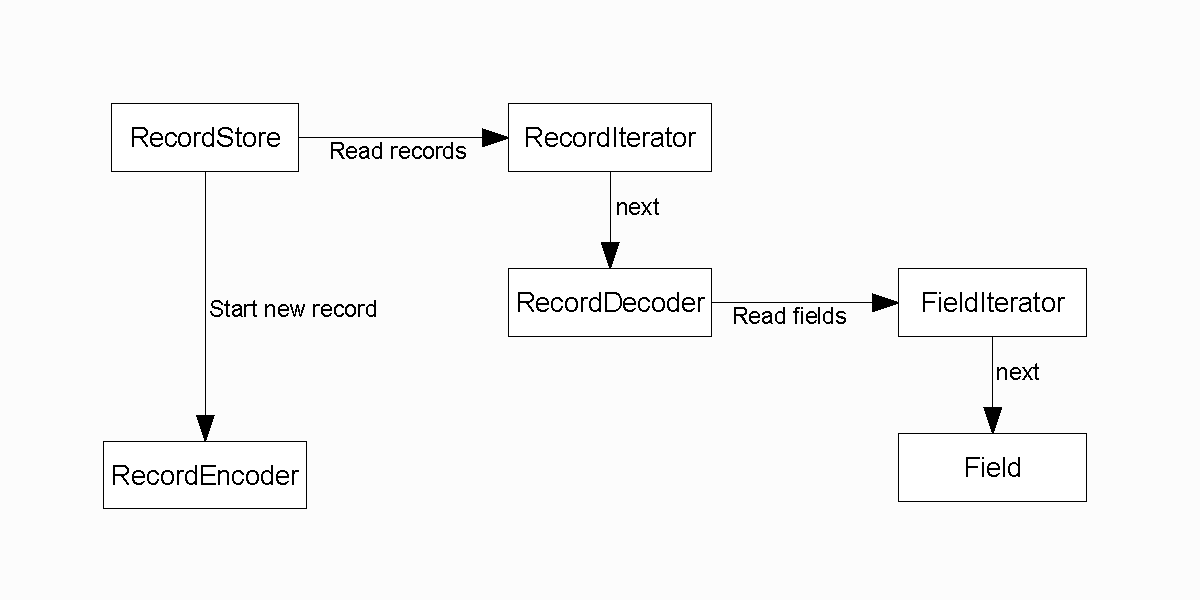
\includegraphics[width=.8\textwidth]{images/hierarchical}
  \caption{The classes for accessing hierarchical data.}
  \label{fig:hierarchical}
\end{figure}

\subsection{Columnar Data}
\label{sec:columnar}

For columnar data we use the same terminology that is used in the Dremel
paper \cite{melnik2010dremel}\footnote{Again, most of the ``classes''
mentioned here are either abstract base classes or interfaces with more
or less trivial implementations.}: A \texttt{Tablet} stores the columnar
data of one partition of a Table. The \texttt{DataStore} manages
the collection of all \texttt{Tablets} of the different tables. Right
now the only implementation of \texttt{DataStore} is the \texttt{LocalDiskDataStore}
which manages the columnar data on the local file system. But it is possible
to implement, for example, a \texttt{HDFSDataStore} that stores columnar
data in a HDFS cluster.

Data is read from a column using a \texttt{ColumnReader} that can be
retrieved from a \texttt{Tablet} instance. \texttt{ColumnWriter} is the
class that is used to write data to a column. At the moment there exist
three implementations of \texttt{Tablet}: \texttt{LocalDiskTablet} that
manages column data on the local file system and
\texttt{InMemoryReadonlyFilesystem} and \texttt{InMemoryWriteonlyFilesystem}
which are used as intermediate tablets for storing query results and
transmitting them over the network.

\subsection{From Hierarchical to Columnar and Vice Versa}
\label{sec:transform}

Transforming hierarchical data to columnar data is done by the column
striping algorithm described in the appendix of the Dremel paper
\footnote{The description in the paper is little
to simplistic though and getting it to work correctly is a bit ``tricky''.}
\cite{melnik2010dremel}
while the other direction is handled by a so-called \term{assembly FSM} which
is also described in the paper.

The field striping is implemented in class \texttt{FieldStriper} which
uses a tree of \texttt{FieldWriter} to to do the actual writing to
the columnar data.\footnote{The implementation of the algorithm is rather
simple with all the previously mentioned infrastructure in place.}

The record assembly code is implemented in \texttt{AssmelbyFSM} and
\texttt{AssemblyFSMNode} which represents on node in the generated FSM.


\section{Query Processing}

When a query arrives at the Coordinator (or SlaveCoordinator) from a client
the query needs to be parsed, analyzed for semanticl correctness,
transformed, sent to lower layers in the network and executed to generate
the result for the client. The interesting parts of this
are examined in the following sections.

The Presslufthammer system can understand queries that look quite like
the pseudo-SQL queries mentioned in the Dremel paper \cite{melnik2010dremel}
and also used by the Google BigQuery system \cite{bigquery}. Our queries
are nevertheless nowhere near as powerfull, since the Presslufthammer system
is still a prototype. 
Some queries that can be processed by the system
are given in \lstref{queries}.

\begin{lstlisting}[basicstyle=\scriptsize\ttfamily,float=htpb,label={lst:queries},caption={Some example queries that can be processed by Presslufthammer.}]
SELECT * FROM Document
SELECT * FROM Document WHERE Document.Name.Language.Country == "gb"
SELECT * FROM Sentence
SELECT * FROM Sentence WHERE Sentence.predicate.arguments.role == "PMOD" OR Sentence.predicate.arguments.role == "NMOD"
SELECT * FROM Sentence WHERE Sentence.predicate.arguments.role == "ADV" OR Sentence.predicate.arguments.role == "DEP"
SELECT Document.DocId AS ID, COUNT(Document.Links.Forward) AS bla FROM Document
SELECT COUNT(Sentence.predicate.text) FROM Sentence
SELECT Sentence.predicate.text, COUNT(Sentence.predicate.arguments.text) FROM Sentence WHERE Sentence.predicate.arguments.role == "ADV"
SELECT Sentence.predicate.text, COUNT(Sentence.predicate.arguments.text) FROM Sentence
\end{lstlisting}

The classes representing a parsed query are in \texttt{query}, they
are \texttt{Query}, \texttt{SelectClause} and \texttt{WhereClause} which
correspond to the respective parts of a query.
The query parser is implemented as an ANTLR \cite{antlr} grammer that directly
generates a \texttt{Query} object as a result of parsing. The parser code
is in \texttt{query.parser}. After parsing the query it must be checked
for semantic correctness, for example it must be checked whether the
referenced table exists and whether the table has the fields mentioned
in the select clauses and where clauses. The semantical analysis code
is in \texttt{query.sema} but as of now it does no analysis besides checking
whether the referenced table exists. (This also means all entered queries
must be correct, otherwise the system will blow up.)

\subsection{Query Transformation}
As mentioned in the Dremel paper \cite{melnik2010dremel} the query must
be transformed before handing it down to child nodes in the network,
and also the query that combines the result from the children must be
rewritten from the original query. This is mostly due to the presence
of aggregation functions. The code that does the transformation of a
\texttt{Query} is in the package \texttt{query.qexec} in the class
\texttt{QueryHelper} it determines the query that must be sent to the child,
the query that is used to stitch together the results form the children
and also some other useful things such as the schema of a query result.

\subsection{Query execution}
The query execution code is in \texttt{query.qexec}. We use the algorithm
from the appendix of the Dremel paper with some modifications to make it
actually work in our system. The basic idea is to advance a set of
\texttt{ColumnReader}s in lockstep and we have class \texttt{Slice} exactly
for doing that and also for writing the current result values to
\texttt{ColumnWriters} that are retrieved from an in-memory result tablet.


\section{Conclusions and Further Work}
  The main difficulty in the network architecture, was the realisation of
  the intermediate layer and the parallel management of multi-part queries
  accross an execution tree.

  Future steps in the development of Presslufthammer could include:
  \begin{itemize}
    \item Implementation of a purely intermediate layer\\
      As described earlier, we already implemented root, client and leaf layers,
      as well as an alternative implementation that mixes intermediate and leaf
      layers. But it appears conceivable, that specialized servers for the
      intermediate layer could provide a valid alternative.
      To evaluate possible benfits or deficits of either solution, this kind of
      server would have to be implemented.
    
    \item Implementation of a distributed storage layer\\
      A distributed storage layer seperate from the leaf layer, could lighten
      storage requirements on leaf servers and allow to reap the benefits of
      such systems, i.e. high availability, redundance and parallel access.
      A popular option could be the HadoopFileSystem.
    
    \item Implementation of a richer graphical user interface\\
      As with all software that includes direct user interaction, an intuitive
      and full featured user interface is highly desirable and critical to 
      said software's success. A possible solution could be a rich web client,
      building on the one we implemented.
    
    \item Improving fault tolerance\\
      Fault tolerance is one of the most important features in a highly
      distributed system, playing a definitive role in the success of systems
      such as MapReduce. Presslufthammer still has a lot of headroom in this
      regard and pursuing improvements appears a worthwhile effort.
    
    \item Testing and Evaluation of distributed execution\\
      In our developement, we did not have the opportunity to test
      Presslufthammer in a truly distributed fashion on multiple nodes in a
      network. Since this would be the natural environment intended for the
      system's operation, it is an obvious and necessary step, going onwards.
    
    \item Performance evaluation at scale\\
      When the system reaches a more mature point in it's development,
      Presslufthammer's performance has to be evaluated to determine it's worth
      and to identify bottlenecks and weak spots within the system. This is
      important to assess the system and to direct further development.

    \item Support of join queries\\
      Google BigQuery gained support for join queries in the most recent
      version and it is surely an interresting task to find out how
      joins over big data can be performed in interactive runtimes.
    
    \item Code generation for query execution\\
      Right now a lot of code is executed for every emitted value in
      query execution, mostly in the presence of where clauses and for
      aggregations. The runtime of those queries could be greatly
      reduced by generating special case code for that and just-in-time
      compiling this code.
    
  \end{itemize}


